\chapter{研究基础和相关工作}

本章首先对视频编码和传输领域的一些基础知识进行概述,作为本文后续内容的铺垫;然后结合本文所涉及的研究内容,对要解决的问题进行详细描述,并对国内外研究现状和已有工作进行分析。

\section{视频的压缩编码}

原始视频信号数据量过于庞大,必须经过压缩才能有效进行存储和传输。视频信号之所以能被压缩是因为其中存在大量冗余信息,包括空间冗余、时间冗余、统计冗余等\supercite{Gao-book-2010}。以仙农信息论\supercite{Shannon-1948}和率失真理论\supercite{Berger-book-1984}为基础,通过预测(如时间预测和空间预测)\footnote{在空域或时域寻找相似信号,用与相似信号的残差来重建当前信号的一种压缩手段。}、变换(如离散余弦变换\supercite{Rao-1990}、哈达玛变换\supercite{Pratt-1969})、量化\supercite{Gray-TIT1997}、熵编码(如变长编码\supercite{Huffman-1952} 、算术编码\supercite{Rissanen-1979})等技术手段,可以去除这些冗余,以一定的失真为代价获得很高的数据压缩比。数字视频压缩编码技术经过了半个多世纪的发展,形成了一系列的国际标准。

最早的视频编码标准通常被认为是由国际电信联盟于1990年制定的H.261\supercite{H.261}。同一时期,由国际标准化组织和国际电工委联合成立的运动图像专家组(Moving Pictures Expert Group,MPEG)也开始了视频相关标准的制定工作,并于1992年推出了MPEG-1\supercite{MPEG1}。此后,以MPEG-2\supercite{MPEG2}、H.263\supercite{H.263}为代表的标准不断演进,大大推动了数字视频产业的发展。时至今日,国际电信联盟与国际标准化组织已经在标准制定方面互相合作,二者共同打造的H.264/AVC视频编码标准在蓝光光碟、高清数字视频光盘(Digital Video Disk,DVD)、数字电视广播、互联网视频共享和在线观看等各个领域都占据了主流地位,普及度极高。虽然意在取代H.264/AVC的新一代视频编码标准HEVC已经于2013年发布,但因为其编解码复杂度高且大多设备和系统尚未支持,所以还处于推广阶段。我国也制定了自己的视频编码标准AVS (Audio Video coding Standard) \supercite{AVS},但影响力远不及国际标准。考虑到上述情况,本文的研究大部分都是基于H.264/AVC及其扩展的;针对新一代视频编码标准HEVC的解码器优化也正是为了促进其推广应用。需要指出的是,随着视频编码技术的逐步成熟和定型,各种编码标准有很多共同点,因此本文的部分研究方法和结果适用于多种标准。

下面依次对H.264/AVC视频编码标准、HEVC视频编码标准、可伸缩视频编码进行介绍,作为后文研究工作的基础。

\subsection{H.264/AVC视频编码标准}

H.264/AVC的设计目标有两方面,一是显著提高编码效率,二是在网络化的趋势下满足对灵活性和可定制性的要求。为此,这一标准相对于之前的标准提出了两个新概念:视频编码层(Video Coding Layer,VCL)和网络抽象层(Network Abstract Layer,NAL)。视频编码层着重于高效地压缩和表示视频内容,而网络抽象层则用于封装视频编码层的数据并提供额外的头信息,使之适用于多样化的传输层测和存储介质(参见图\ref{fig:02}\supercite{H.264-Overview})。

\begin{figure}[h]
	\centering
	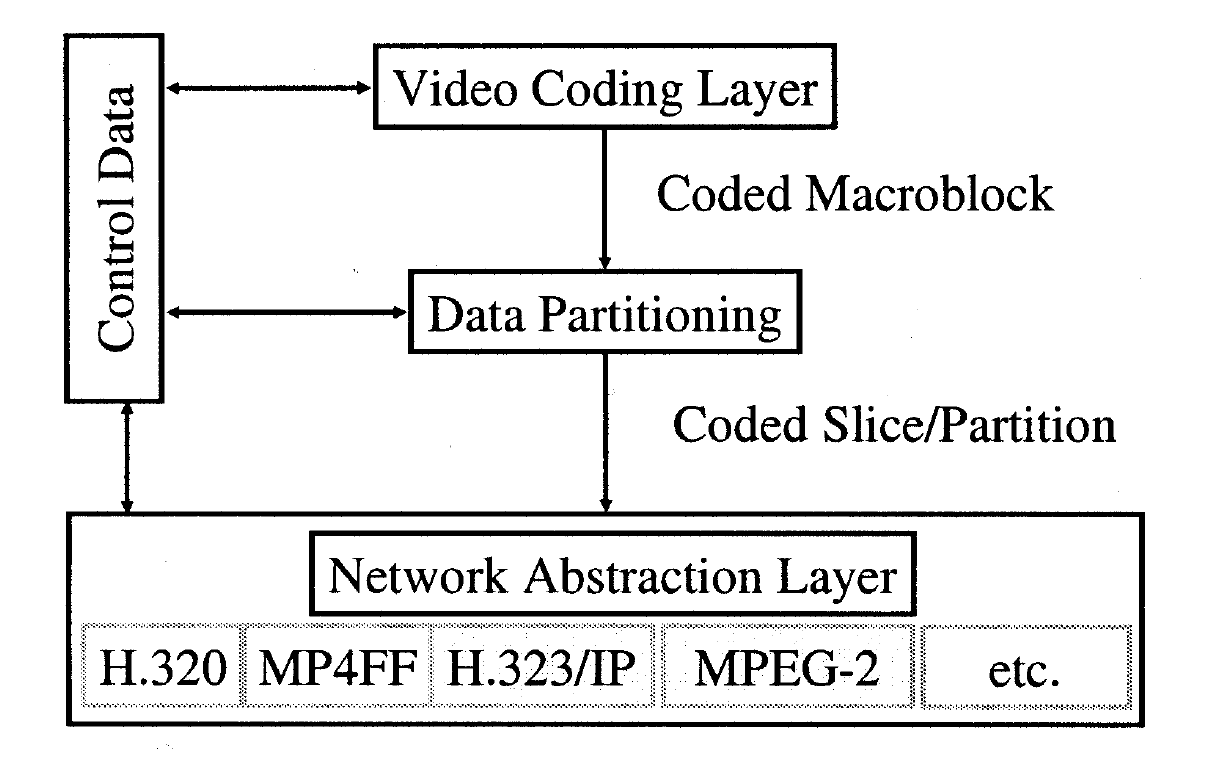
\includegraphics[width = 0.6\linewidth]{clip/02.png}
	\caption{H.264/AVC编码标准的结构\label{fig:02}}
\end{figure}

图\ref{fig:02}中,H.320是国际电信联盟制定的关于在综合数字交换网上进行视频会议的标准,H.323则是其在IP电话方面的标准,MPEG-2规定了音视频文件存储格式。可见,经过NAL层的抽象,H.264/AVC编码得到的码流可以灵活适应各种应用。下面,分别对VCL和NAL进行介绍。

VCL层的目标是高效率地表示视频内容。与其他视频编码标准一样,H.264/AVC的VCL层采用了基于块的混合视频编码框架,如图\ref{fig:03}\supercite{H.264-Overview}所示。

\begin{figure}[h]
	\centering
	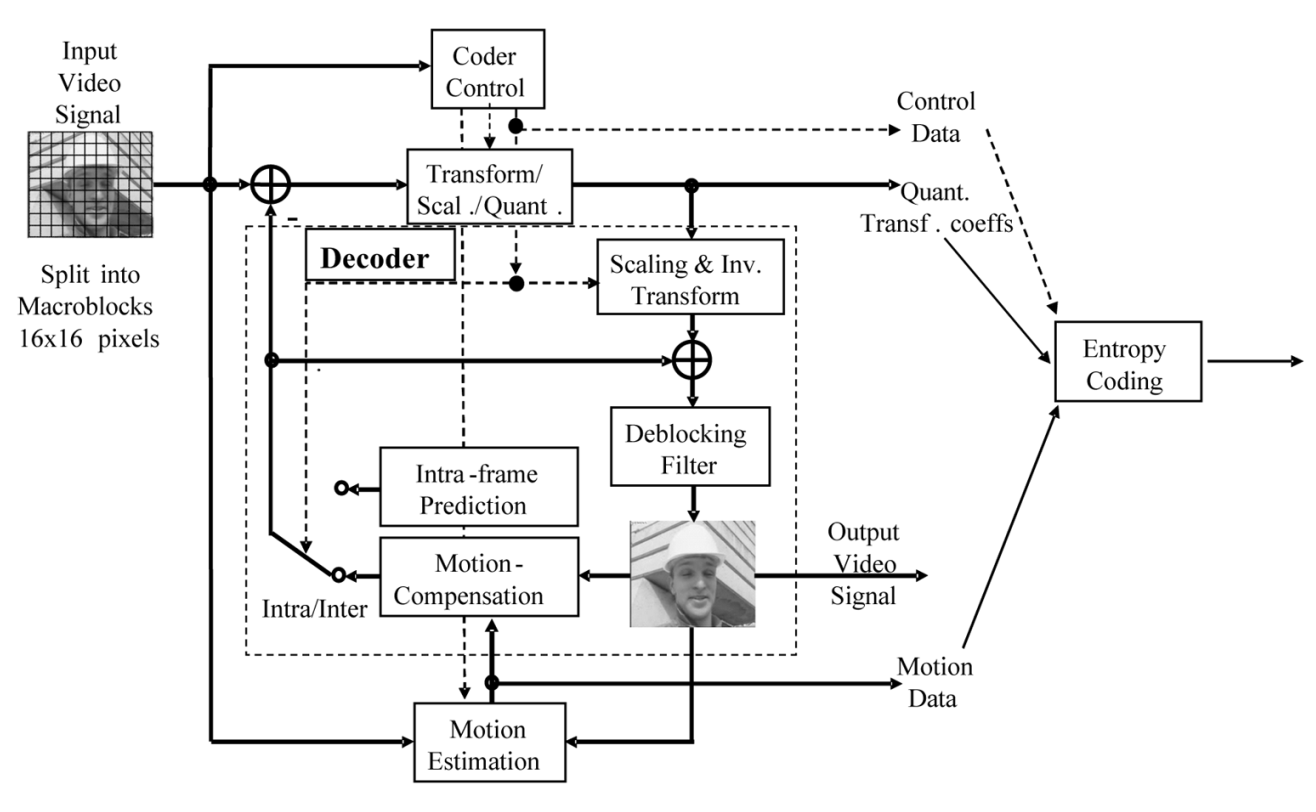
\includegraphics[width = 1.0\linewidth]{clip/03.png}
	\caption{H.264/AVC的VCL层编码框架\label{fig:03}}
\end{figure}

所谓“基于块”,是指将原始图像数据分成16x16大小的宏块(Macro Block,MB),接下来的编码过程将以宏块为基本单位。对每一个宏块,先进行时间或空间预测;预测得到的残差数据进行类似于离散余弦变换(Discrete Cosine Transform,DCT)的整数变换,然后对变换系数进行量化、重排、熵编码,最终形成比特流。

虽然这样的编码流程与之前的编码标准并无二致,但由于H.264/AVC对各个阶段进行了精心设计,并将灵活性和适应性贯穿于整个编码过程,使得其编码效率大大提高。以下仅着重分析H.264/AVC相对于之前标准的改进之处。

预测分为帧内预测和帧间预测,目的分别是去除空间和时间冗余。在H.264/AVC中,预测时可将一个宏块进一步分为小的子块进行,最小可以分成4x4的小块。标准还提供了多达9种的预测模式,从而能够更精细地利用局域特性。而对帧间预测,H.264/AVC除支持单向和双向预测之外,每个方向还允许选用多个参考帧。在运动向量的准确度上,新的标准允许精确到1/4像素,而且还允许跨越边界的值(采用外推插值技术)。

对预测残差进行变换可以进一步去除空间相关性。考虑到精细的预测模式已经很好的去除了相关性,H.264/AVC一改之前标准以宏块为单位的DCT变换,采用了更小的变换块(4x4)。而且对于相对平滑的色度值(YCbCr/YUV中的U、V),还对每个宏块中的4个4x4子块变换后的直流系数又做了一次哈达玛变换。小尺寸块的变换大大减小了计算复杂性。当然,H.264/AVC也支持将变换块扩展成16x16大小。

H.264/AVC提供了两种熵编码方法CAVLC(Context Adaptive Variable Length Coding)和CABAC(Context-based Adaptive Binary Arithmetic Coding)来去除量化后系数(以及其他一些参数)的统计冗余。它们都是上下文自适应的,前者为可变长编码,后者为二进制算术编码,后者计算较复杂但压缩率高,前者反之,可根据应用场景配置不同的算法。

以上只选取VCL的部分特性进行了简述。除了所提到的方面,H.264/AVC还包含更多可由编码器选择的配置。这样不仅能够更有针对性地去除冗余、提高编码效率,而且也增加了该标准的普适性、灵活性和可定制性。正因为如此,能够在其基础上方便地进行扩展。

VCL编码得到的比特流送去NAL层进行封装。NAL的设计目标是提供网络友好性,使得VCL数据在不同系统中的使用可以简单而高效地定制。我们后面将看到,在H.264/AVC基础上扩展得到的码流能与普通的H.264/AVC码流无缝兼容,很大程度上得益于这种网络抽象层机制。

网络抽象层的基本概念和语法结构是NAL 单元(NAL Unit,NALU)。这是一种由整数个字节组成的数据包。一个NALU以1字节的头信息起始,之后是不定长度的载荷。参见表\ref{tab:nal}。

\begin{table}[h]
\centering
\caption{H.264/AVC中的NAL单元结构}
\label{tab:nal}
\begin{tabular}{|*{11}{p{1.2cm}<{\centering}|}{p{1.2cm}<{\centering}}}
	\hline
	\multicolumn{8}{|c|}{NALU头字节} & \multicolumn{4}{c|}{NALU载荷} \\ \hline
	F & \multicolumn{2}{c|}{NRI} & \multicolumn{5}{c|}{TYPE} & \multicolumn{4}{c|}{......} \\ \hline
\end{tabular}
\end{table}

NALU字节头包含禁止位 (F,1bit) 、重要性指示位 (NRI,2bit) 、NALU类型 (TYPE,5bit) 三方面信息。其中禁止位规定为0,重要性指示位在一定意义上表示该NALU的重要程度,而NALU类型则表明该NALU中携带的是什么样的载荷。

在H.264标准中,NALU类型的0~12已被规定了用途,13~23被保留用于以后可能的标准扩展,24~31不做规定,可根据应用场景定制。按照NAL单元中载荷的不同,将其划分为两类:VCL单元和non-VCL单元。前者主要包含来自VCL的图像样本值编码数据,后者主要含有图像或序列参数集、补充增强信息(Supplemental Enhancement Information,SEI)等解码多个VCL单元所共用的一些重要数据。这种机制不仅能节省开销,也便于将重要数据通过更可靠的信道传输。对如何使用SEI来存储和传输额外的信息,后文在码流截取部分会有涉及。

\subsection{H.264/AVC的可伸缩扩展}

可伸缩视频编码(Scalable Video Coding,SVC),简言之,就是在视频编码时生成一个包含不同层次信息的码流。从这个单一码流中,我们能够方便地丢弃一些数据,得到不同码率的多个码流,从而解码出在空间大小、帧率、画面质量等方面可伸缩的视频。虽然之前的标准也考虑了对可伸缩性的支持,但目前提到可伸缩视频编码,大多指的是H.264/AVC的可伸缩扩展。

SVC在传统编码的基础上引入了“分层编码”的概念。即对数据源一次编码得到的码流中,含有一个或多个的“层”。其中最低分辨率、最低帧率和最差图像质量的部分称为基本层,除此之外为增强层。增强层对应着更高的分辨率、帧率和图像质量。这样的码流能够提供在空间、时间、质量(或信噪比)等方面的伸缩性。当终端没有能力播放增强层或者网络无法承担高码率时,可伸缩码流的增强层部分会从比特流中移除,只有基本层数据被传送到终端解码器。
SVC编码标准得益于H.264/AVC灵活的编码逻辑结构,也继承了H.264/AVC中许多良好设计的编码工具。SVC不仅在编码效率和复杂性上与单层编码增加不多\supercite{SVC-Performance},并且完全兼容H.264/AVC。以下结合传统编码框架,在H.264/AVC的基础上,对SVC可伸缩性的实现原理进行概述。

具备时间可伸缩的码流能够根据需要动态改变视频帧率。在H.264标准中,把用于解码一帧的多个NAL单元称为一个AU(Access Unit)。SVC就是通过丢弃AU来降低帧率。时间可伸缩的实现不需要对H.264做任何增加,只需采用一种称为“层次化预测结构”的技术。

\begin{figure}[h]
	\centering
	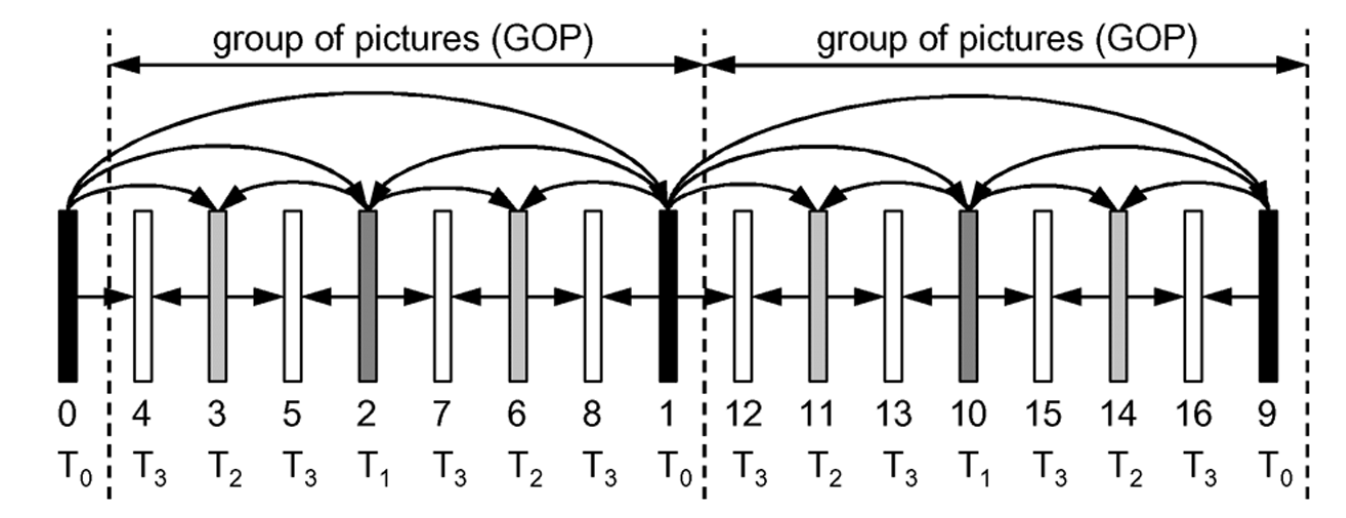
\includegraphics[width = 1.0\linewidth]{clip/04.png}
	\caption{H.264/SVC中通过层次化预测实现时间可伸缩\label{fig:04}}
\end{figure}

图\ref{fig:04}\supercite{SVC-Overview}说明了通过层次化预测来实现时间可伸缩的原理。图中一个AU下面的数字表示其编码顺序,数字下面的符号$T_i$表示其属于第$i$时间层。增强层($i>0$)的帧被编码为B帧(即参考其前后的帧进行双向预测),而且只参考较低层的帧。这样的结构下,低层的AU可以不依赖于高层,即任一较高层及其以上各层的AU可以被丢弃而不影响解码,以此实现帧率的伸缩性。需要说明的是,此例中这种“层次化B帧”的结构会带来编解码时延,且仅限于1:2伸缩比,这些不足均可通过仔细设计层次化预测结构而改善。

空间可伸缩是指视频大小的改变。空间可伸缩的实现比较复杂,需要在H.264中引入分层编码。每个分辨率都对应一个H.264编解码层,称之为“dependency layer”,由DID(Dependency ID)标记。每个层都需要不同尺寸的输入图像,这一般由最高分辨率的图像下采样得到。每层的运动补偿和帧间预测都和单层H.264编码一样,然而由于表示的是同一图像,各层之间必然有很强的相关性。SVC规定了各层之间的预测机制,称之为“层间预测”,以此来提高编码效率。

质量可伸缩顾名思义就是视频各帧的图像质量可变。这是通过丢弃一个AU中的一些质量精细化NAL单元来实现的。具体操作时,给一个AU内的每个NAL单元打上质量层标记QID(Quality ID),可以将QID高于某个值的所有NAL单元丢弃,剩下的即可组成较低质量的码流。

以上分析的主要是在VCL层实现可伸缩编码的原理,可以看到多处涉及对特定NAL单元的取舍。这就需要对H.264的NAL层进行扩展从而能够在码流中标记和传送特定的可伸缩性信息与数据。

在前面介绍H.264/AVC时曾提到,NALU头字节中的NAL类型(nal\_type)在13~23的取值留作扩展;SVC就增加了一些扩展的NAL类型。nal\_type=20的单元为新增的VCL单元,包含的是SVC中增强层的编码数据;nal\_type=14为新增的SVC前缀单元,它可能是VCL的也可能是的non-VCL的,取决于紧接着它到来的NALU。nal\_type=15的NALU用来传送SVC特有的图像参数集。对于这些新增类型的具体分析可以参见相关文档\supercite{SVC-Interface}。

普通H264解码器遇到nal\_type大于12的单元会忽略之,但能成功解码基本层,因此SVC可与之兼容。而支持SVC的解码器将对类型为14、20的NALU进行利用,实现可伸缩性。与普通H.264的NALU不同,类型为14、20的NALU并非只有1个头字节,而是扩展为4字节的头。如图\ref{fig:05}\supercite{SVC-Interface}所示。

\begin{figure}[h]
	\centering
	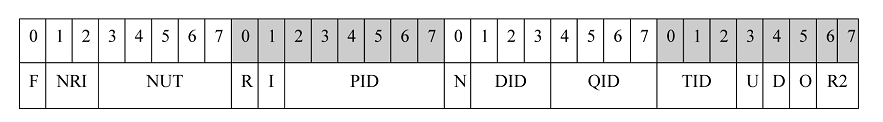
\includegraphics[width = 1.0\linewidth]{clip/05.png}
	\caption{4字节的SVC NAL单元头结构\label{fig:05}}
\end{figure}

可以看出,其中除了与普通NALU一致的第一字节,还包含了空间、时间和质量层的标志(DID、TID、QID)以及其他一些用于提供可伸缩性的信息。

根据以上分析,可在标准H.264编解码器的基础上扩展得到SVC编解码器。无论H.264还是SVC,在标准文档中都只对码流的语法语义和解码过程做了规定,换句话说:对编码的过程不做限制,只要得到符合标准的码流即可。因此编码器的程序实现可以多种多样,而解码必须与标准一致。
 
SVC标准由国际电信联盟与国际标准化组织的专家组成的联合视频小组制定。该组织在标准形成过程中还开发了一个官方的参考软件,称为JSVM(Joint Scalable Video Model)\supercite{JSVM}。该软件完整实现了SVC的编解码过程。虽然该软件未做优化很难实用,但由于其囊括了SVC标准中的几乎所有特性且清晰逻辑、配置简单,比较适合学习参考,以及作为研究性的实验平台。因此,几乎所有的学术工作都是基于JSVM参考软件,在其上实现自己的算法并与内置的算法进行对比,体现其效率的提升。本文的研究中也采用了JSVM作为比较对象。

\subsection{HEVC视频编码标准}

作为新一代国际视频编码标准,HEVC的目标是相比H.264/AVC提升一倍的编码效率。HEVC仍然沿用了传统的基于块的混合编码框架(如图\ref{fig:17}\supercite{HEVC-Overview}所示),但提出了新的视频内容表示单元并引入了更加复杂的编码工具。这些新的工具目的在于提高编码效率,尤其是针对日益增多的大分辨率视频。最终发布的HEVC标准在客观和主观测试方面都已经达到了预期的目标。

\begin{figure}[h]
	\centering
	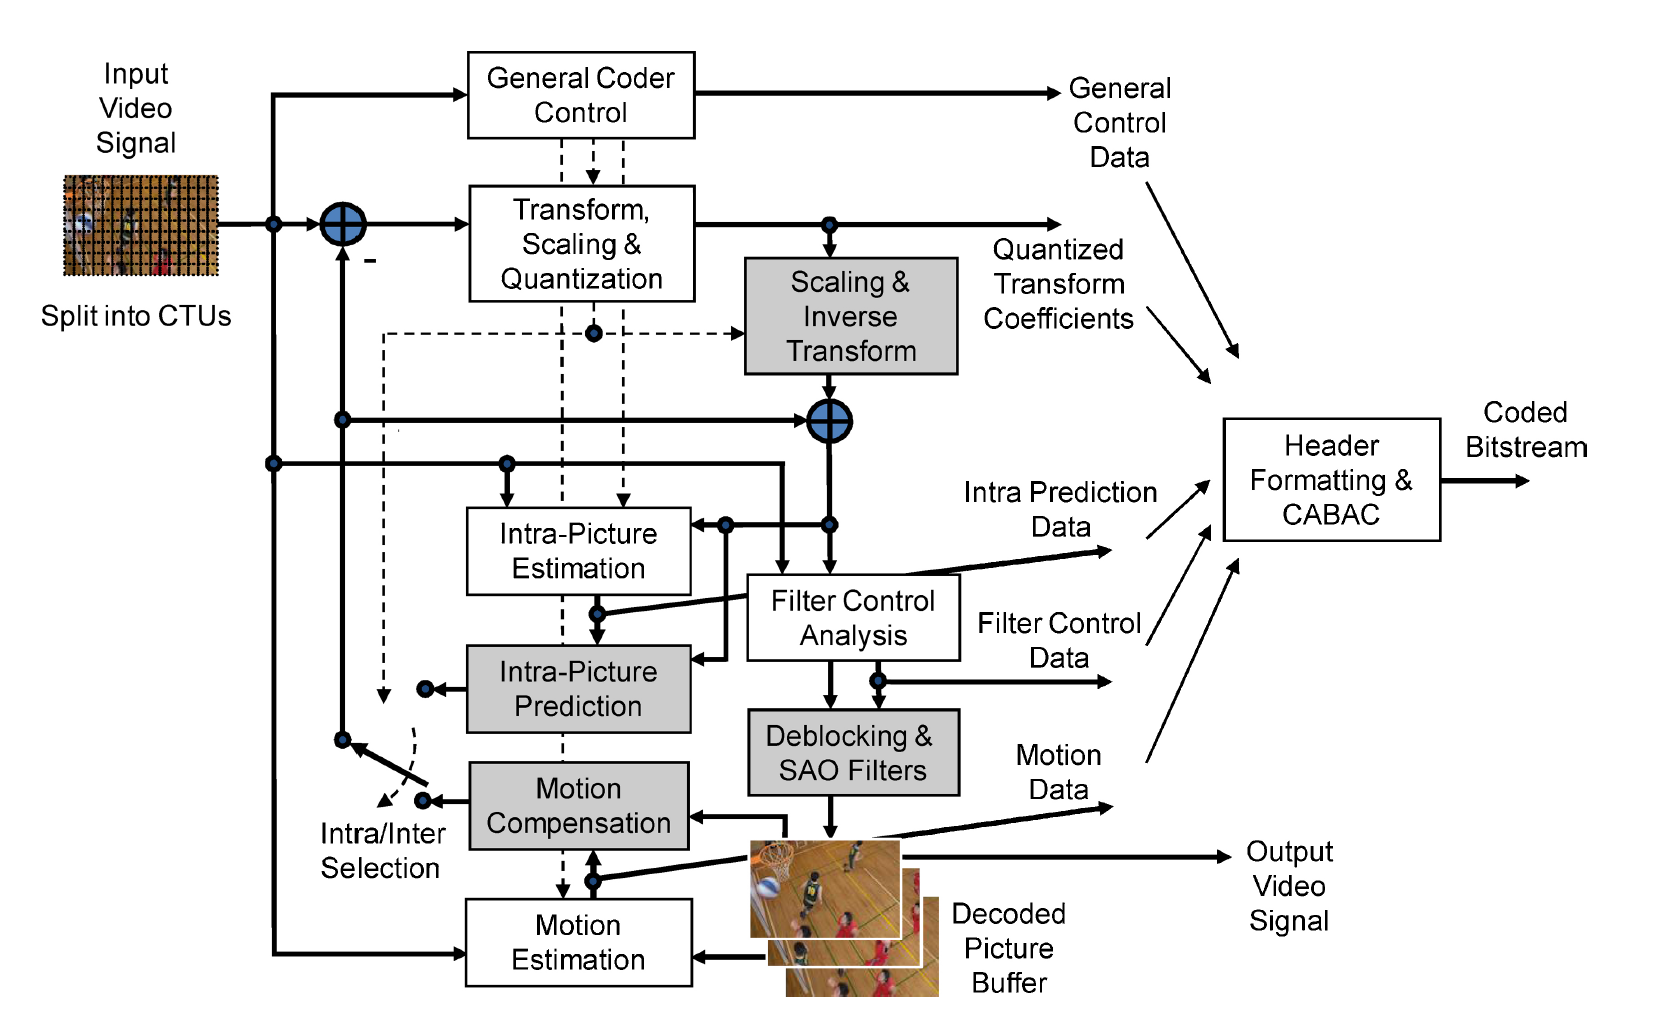
\includegraphics[width = 1.0\linewidth]{clip/17.png}
	\caption{典型的HEVC编码器结构\label{fig:17}}
\end{figure}

在H.264中,编码的基本单位是宏块(Macro Block,MB),一个宏块可以分为子宏块和块(Block)。HEVC对这种区域层次划分结构作了扩展,支持从128x128到8x8五级大小的编码单元。HEVC中的操作单元有三种,分别是编码单元(Coding Unit,CU),预测单元(Prediction Unit,PU)和变换单元(Transform Unit,TU),对应了编码的不同阶段。CU是对视频内容进行四叉树形式的划分。对一个序列在序列参数集中指定一个最大CU。最大CU可对称划分为4个子CU,最多可划分5层,可能形成128x128(最大CU)、64x64、32x32、16x16、8x8五种大小的编码单位。最终的子节点的CU进行帧内或帧间预测时被作为一个PU,所有预测相关的信息(包括预测模式、帧内预测方向、帧间预测的参考索引等)都是以PU的形式组织和传送的。根据不同的预测模式,PU内部可以进一步划分,而且这种划分可以不是对称的,这就为选择最好的预测方案提供了可能。在对残差进行变换和量化时,HEVC提出了TU的概念。一个变换单元可以与它所属的CU大小一致,也可以更精细,从而为率失真优化过程提供了更多选择。值得注意的是,TU可以包含多个预测区域,也就是说变换可以针对不同预测得到的残差进行,这对某些复杂纹理特征可以取得更好的压缩效果。

由于新的表示单元把预测、变换这些阶段独立开来,使得整个编码过程增加了更多灵活性。此外,上述单元定义使得语法元素的设计可以不受块大小的影响,采用一致的方案(在H.264中,一些语法元素的设计对于不同的块大小是不一样的),这可以简化编码规范和解码时的分析过程。

除了表示单元的变化,HEVC对H.264/AVC中的编码工具进行了扩展,或引入了一些新的技术来提高性能。以下对其中一些新特性分类作介绍。

帧间预测:运动估计的精度在原来1/4像素的基础上增加了1/12像素的精细化选项,以得到更准确的运动向量;运动校正时的插值过程改用基于DCT的插值滤波器,任意精度和任意大小范围的插值滤波参数都可以根据公式方便求得,而且非整数位置的像素值均直接由整数位置像素值计算出来;采用了更先进的运动向量预测,即预测参考可以从多个候选者中择优,不像H.264是特定的。

帧内预测:帧内预测方向扩展为任意的,不再局限于H.264的9个特定方向,以适应大分辨率视频的特点;对每一个PU,预测得到的值可以进行平滑处理从而更利于接下来的残差变换;新标准的预测机制还考虑了不同颜色分量之间的相关性、像素模板匹配、预测结果与原像素值的加权组合等多种因素,共同提高帧内预测的效果。

空间变换:仍然采用类DCT的整数变换,但考虑到新的优化算法的出现以及对编码大分辨率视频的需求,变换块的大小增加至16x16、32x32甚至64x64;而且在整数变换之后,还可以增加一个旋转变换来更好压缩某些强对角分量的残差。

环内滤波:为消除块效应、降低重建图像和原图的误差,需要对重建图像做去块滤。新标准的去块滤波在H.264的基础上增加了随CU的适应性,即可对不同单元选择打开或关闭这一滤波过程。此外,为进一步消除误差,还引入了其他纠正措施作为后处理过程。

熵编码:主要还是H.264中的CABAC编码,但一方面增加了对不同语法元素的适应性,另一方面对编码前的系数扫描过程也提供了多种模式(Zig-Zag,横向,竖向)供择优选取。

采样自适应偏移(Sample Adaptive Offset,SAO):增加到了环内去块滤波之后,旨在进一步改善重建图像质量。

从最早的H.261到现在的H.264/AVC、SVC,再到最新的HEVC,一系列视频编码标准的制定和推广过程不仅促进了产业发展,还在以下两个方面催生了大量的学术研究成果。一是对信源编码理论及应用的研究,包括对图像视频中不同信源的概率分布建模\supercite{Birney-TIP1995, Lam-TIP2000, Sharifi-TCSVT1995, Kamaci-TCSVT2005},对特定信源分布下率失真函数和量化器性能的分析\supercite{He-TCSVT2001, Gary-TIT1996, Gary-VCIP2005},基于率失真分析和估计来改进编码中的率失真优化和码率控制过程\supercite{Gary-SPM1998, Lin-TCSVT1998, Sun-TCSVT2006, Lee-TCSVT2014},等等;这些研究旨在不断提高压缩效率和编码器性能,是视频产业链上后续相关环节的基础。二是视频编码与网络传输相结合的研究\supercite{Sun-book-2001},包括在Internet上传输视频\supercite{Wu-TCSVT2001, Conklin-TCSVT2001},采用可伸缩视频编码以应对网络异构和拥塞导致的带宽波动\supercite{Wu-IEEE2001, Ohm-IEEE2005},等等。这方面的研究则直接推动了视频流媒体应用不断改善和蓬勃发展。本文的工作主要偏向于上述第二方面。下面对视频流媒体相关知识进行介绍。

\section{视频文件的流式传输}

流媒体系统之所以能够在不必下载完整音视频文件的情况下进行播放,主要是因为采用了流式传输。流式传输的对象是存放在服务器上的流式文件。生成流式文件是流媒体系统的起点。流式文件经过了特殊编码,使其适合在网络上边下载边播放。对于编码压缩好的视频文件,需要将数据分成适当大小的分组并考虑差错恢复功能,此外一般还要加入特定的时间戳和索引(hint或index)信息,用于提供如快进、后退和随机访问等控制功能。上述过程称为媒体文件的流化。流化得到的流式文件存放在服务器上等待传输。

流式传输是流媒体系统的关键。通常流式传输可以分为两种:顺序流式传输和实时流式传输。顺序流式传输虽然也能边下边播,但用户只能观看已下载的部分,不能跳到未下载的前面部分。这种流式传输方式通过HTTP即可实现,不需其他特殊协议,但其功能和特性也不够灵活。与之相对应的是实时流式传输。这种方式允许用户对媒体流的发送进行更多的控制,可随机访问前后内容。相应地,这种传输方式也需要特定的服务器和特殊的协议。图\ref{fig:10}给出了典型的流媒体视频点播系统的基本框架。

\begin{figure}[h]
	\centering
	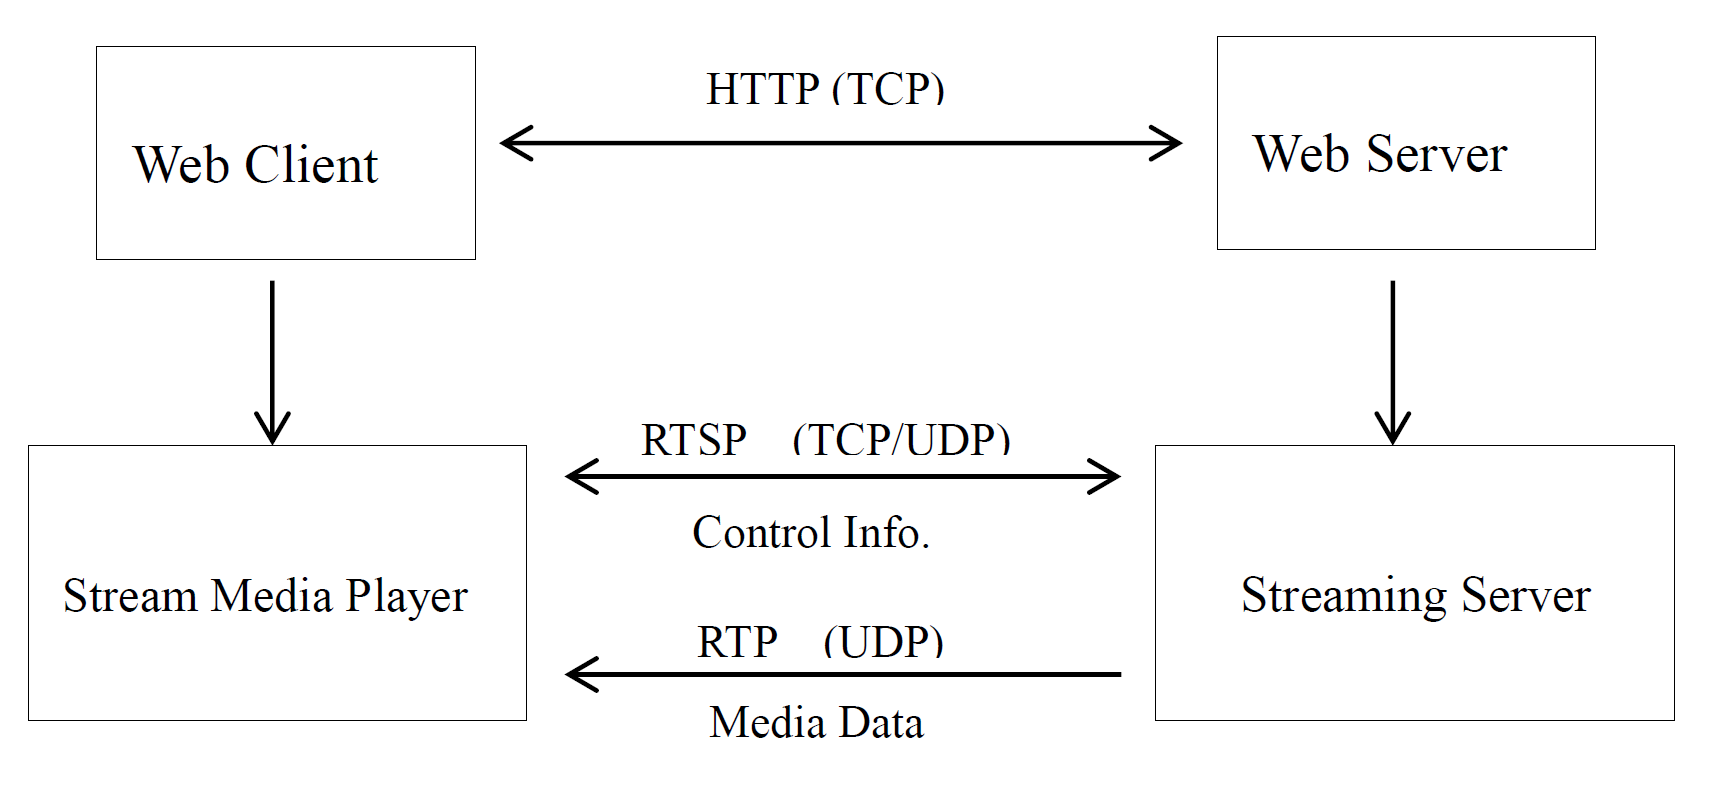
\includegraphics[width = 1.0\linewidth]{clip/10.png}
	\caption{典型的流媒体应用框架\label{fig:10}}
\end{figure}

图\ref{fig:10}可见,通过流式传输播放在线视频的一般过程如下:
\begin{enumerate}
\item 用户根据观看意愿检索和选择视频;在Web浏览器与Web服务器之间通过HTTP/TCP进行通信。
\item Web浏览器利用从服务器得到的参数对客户端的流媒体播放起进行初始化;这些参数包括流媒体服务器地址、目录和媒体文件信息等。
\item 播放器与流服务器之间运行实时流控制协议(Real-Time Streaming Protocol,RTSP),进行A/V 数据传输的控制,如准备、开始、暂停、后退等。
\item 流服务器使用实时传输协议(Real-time Transport Protocol,RTP)将媒体数据传送给客户端,数据抵达时即可解码播放。
\end{enumerate}

流媒体是面向网络的应用,既需要终端软件,也需要传输和控制协议。本节剩余部分中,首先介绍流媒体传输用到的几个典型协议,然后介绍代表性的流媒体服务器。

\subsection{典型的传输协议}
\label{subsec:protocols}

实时流协议RTSP是一种应用层协议,其目的是为了在IP网络中有效传输流媒体数据。RTSP本身并不发送媒体数据内容,它主要起到建立流和控制流的作用。RTSP类似于HTTP,在客户端和服务器之间发送请求和回应。一般会有以下交互:
\begin{itemize}
\item OPTIONS: 客户端询问服务器有哪些操作,服务器进行回应,列出可用的方法。
\item DISCRIBE:客户端向服务器请求描述信息,服务器以会话描述协议(Session Describe Protocol,SDP)的形式返回该信息,包括音视频的编码类型、参数,控制通道等等。
\item SETUP:客户端在得到媒体信息后建立流;对音频、视频需要分别建立。
\item PLAY(类似的有PAUSE、SCALE等):开始播放媒体(或进行控制)。服务器在收到PLAY后会开始以RTP协议发送媒体数据包。
\item TEARDOWN:客户端请求关闭流。
\end{itemize}

可见,RTSP只在播放流媒体之前和结束时发挥作用。实际传输数据采用的是实时传输协议RTP。

实时传输协议负责传输媒体数据。它是单向的,将流媒体内容以包的形式从服务器发送至客户端。RTP包由头信息和载荷组成\supercite{RTP}。包头中提供了版本号、有效载荷类型、时间戳、序列号等信息,并且允许扩展。包的载荷则是实际的音视频编码数据。接收端解码时必须知道RTP载荷中数据的编码方式,包头中的有效载荷类型即标识了这一信息。有效载荷类型域共7bit,可表示多达128种载荷。除了标准中指定的类型外,还可以进行扩展。

可以用指定有效载荷类型的RTP包来表示所传送数据的编码方式为H.264。此时,RTP载荷(payload)将呈现为H.264定制的结构\supercite{RTP-H.264}。H.264的一个NAL单元大小不定,有时会超过一个RTP包的容量(受限于RTP下层协议的包大小,如UDP);有时又较小,可将多个NAL单元封装在一个RTP包中。为此,针对H.264的RTP载荷将第一个字节作为头字节来标记上述的分拆和组合。事实上,H.264的RTP载荷的第一字节采用的结构与NAL单元的头字节相同,并且各个比特的意义也一致。其中后5bit表示该RTP包中的NAL单元的类型,若为0~23则表示H.264标准的一个完整NAL单元,大于24的被用来表示拆分或组合NAL单元。

RTP为包括H.264在内的不同标准流媒体数据提供了有效的传输支持。但它却是不可靠的,它本身没有任何错误检测或拥塞控制机制,因此无法提供QoS(服务质量)保证。RTP底层可以使用UDP也可以使用TCP,但大多采用的是UDP。而且RTP一般与下面介绍的实时传输控制协议(Real-time Transport Control Protocol,RTCP)配合使用。

实时传输控制协议RTCP被设计用来监测流媒体传输质量并在RTP会话参与者之间传递信息。RTCP包可携带不同类型的信息,其中最典型的是接收者报告。这种RTCP包由接收者向服务器发送,报告其收到的RTP包数目、丢包数、包的抖动、延时情况等。这相当于提供一种反馈信息,发送端应用程序可以利用这些信息做出调整,如改变发送速率等。一般流媒体软件都会利用RTCP来控制和保证传输质量。

\subsection{流媒体服务器}

实用的流媒体系统离不开服务器端软件和客户端播放软件。客户端软件主要是支持播放流媒体,为此除了普通媒体播放功能,还需要实现RTSP、RTP等网络协议,但总体来说比较简单。下面着重对流媒体服务器端程序进行介绍。

在流媒体服务器上运行的程序负责响应连接请求,从存储系统中取出音视频数据并以流式传输的方式发送给客户端。完整的流媒体服务器平台需提供会话服务、内容服务、流服务、媒体数据存储管理等(参见图\ref{fig:11})。目前市场上应用较多的流媒体技术和平台主要有三种:RealNetworks公司的RealSystem,微软公司的Windows Media,以及苹果公司的QuickTime。它们分别有各自的流媒体服务器和播放器。前两家的产品都只有闭源的商业版,而苹果公司的流媒体服务器除了商业版本外,还同时提供开源的版本,称为达尔文流媒体服务器(Darwin Streaming Server,DSS)\footnote{http://dss.macosforge.org/}。该服务器经常被用来做相关的研究测试\supercite{Huang2004},本文在视频点播方面的码率自适应研究就是基于它进行的。

\begin{figure}[h]
	\centering
	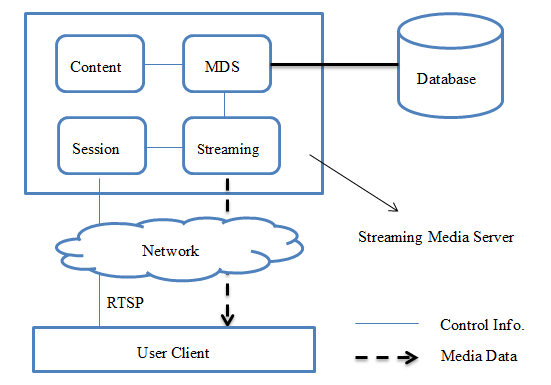
\includegraphics[width = 0.9\linewidth]{clip/11.png}
	\caption{流媒体服务器的组件及其与外界的交互\label{fig:11}}
\end{figure}

原本的达尔文流媒体服务器是不支持SVC的,为了本文的研究和实际的应用,可以在其源代码上修改使其增加对SVC的支持。达尔文流媒体服务器包含多个工程,其中负责流发数据的主要集中在StreamingServer工程中。在这里,由RTSP协议与客户端建立连接会话,并在客户端的SETUP命令下建立多个音频和视频的流,然后由RTP协议向客户端发送数据。每个会话对应一个RTPSession类,每个流对应一个RTPStream类,RTPStream类的Write函数起到实际的发送数据功能。实现对SVC的支持主要是在此类中改变向流中写数据的逻辑。当然,前提是数据的来源必须是SVC的。

达尔文服务器处理的媒体数据来源于特定的MP4文件。正如前文提到的,与本地播放的普通MP4文件不同,用于流式传输的MP4必须经过hint处理(即流化)。流化后的MP4文件不仅包括对应音、视频的audio track和video track,还包括一个hint track,其中信息用于流式传输。SVC的MP4文件区别于非SVC的地方就是在hint track中有SVC伸缩层的数目信息,因此要采用特定的SVCCreator工具来打hint。SVCCreator在打hint时会将SVC视频流所支持的空间、时间、质量层数目写入hint track。这样流化得到的MP4文件就是支持SVC的,可送给达尔文服务器。达尔文服务器在接受到客户端的DESCRIBE命令(以RTSP发送)后,会解析MP4文件中的相应媒体信息,以SDP的形式发给客户端。SDP中包含了音视频的参数,其中可以任意添加参数项。我们在描述视频的参数中加入svclayercount这一项,把从hint track读到的空间、时间、质量层数目告诉客户端。这就使得客户端可以主动设置想要接收的层。这只是提供一种支持,客户端也可以完全不主动设置,服务器会根据网络状况自动调整发送的增强层数据。具体如何调整,就是本文所要研究的码率自适应问题。

\section{可伸缩视频码流截取}

\subsection{问题描述}

可伸缩视频码流截取使视频码率可以动态调整,是基于可伸缩视频编码进行自适应流媒体传输的基础。所谓码流截取,是指从一个完整的码流中抽取所有数据包的一个子集,得到一个更低码率的子流的过程。图\ref{fig:Bitstream-Extraction}展示了一个可伸缩视频码流的结构,以及从中截取子流的一种可能的方式。
可以看到,该码流中的数据包被分为了不同的层。时间层(T0~T3)反映了各帧之间的参考或依赖关系。图形上方的箭头从被参考帧指向参考它(也就是依赖于它)的帧。质量层(Q0~Q2)反映了一帧之内的视频质量伸缩性。处于高层(也就是Q1和Q2层)的数据包可以被部分丢弃从而实现码流截取。图中的虚线表示了一个截取的例子。虚线上方的数据包全部被丢弃,只有虚线下方的数据包保留在截取出来的子流中。

\begin{figure}[h]
\centering
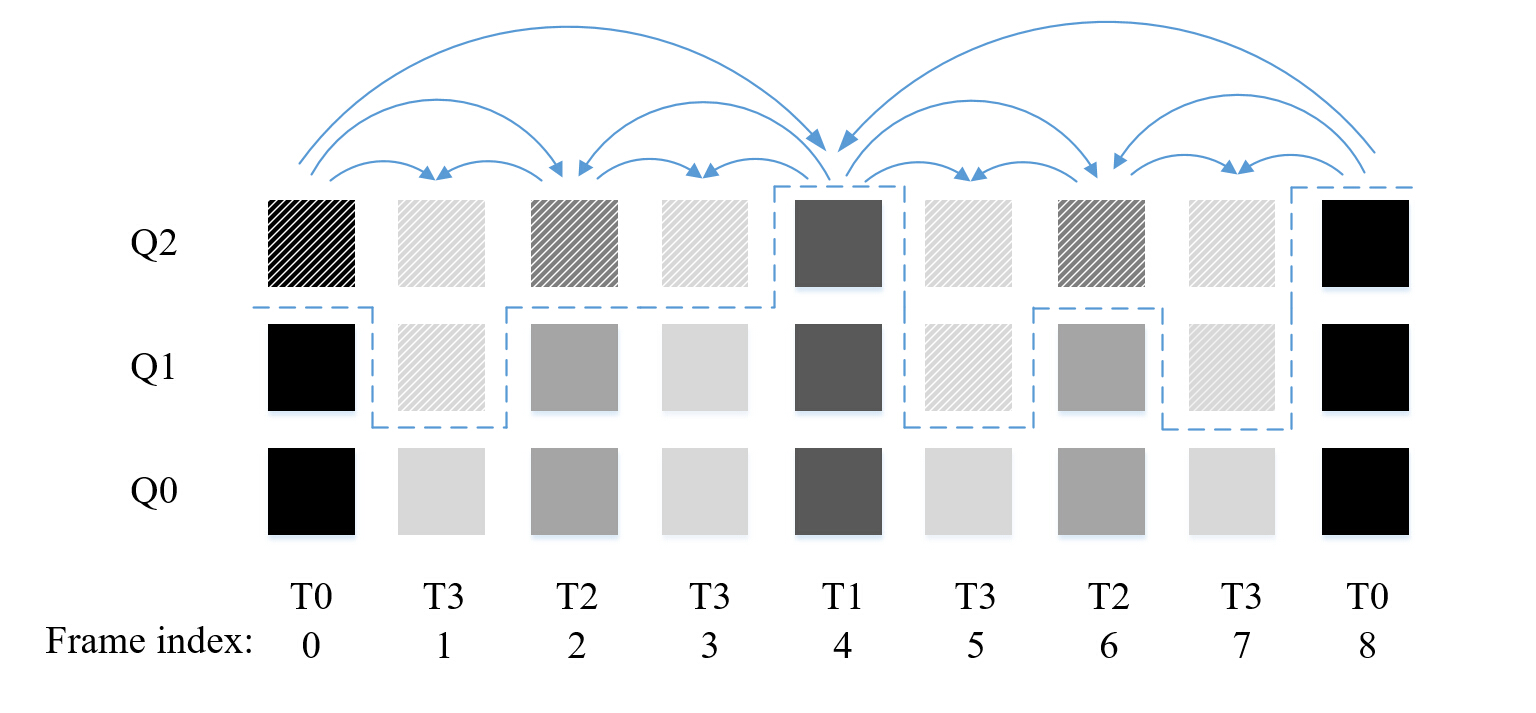
\includegraphics[width = 0.9\linewidth]{./figures/Bitstream-Extraction.jpg}
\caption{可伸缩视频码流截取示意图\label{fig:Bitstream-Extraction}}
\end{figure}

容易发现,可伸缩视频码流截取从本质上来看其实是一个组合优化问题。在所有的数据包中,我们希望在给定的码率限制下,选出一个最优的数据包组合,使得它们构成的子流具有最大的视频质量。如果用$R_T$表示码率限制,$\theta$表示某种截取方案,那么码流截取问题可以用下面的式子表示:
\begin{equation}
{\theta}^* = \mathrm{arg} \min \limits_{\theta \in \Theta} D(\theta), \quad  \mathrm{s.t. } \quad R(\theta) \le R_T.
\end{equation}

其中$D(\theta)$和$R(\theta)$分别表示这种截取方案下对于的失真和码率。

更准确地说,这个问题与大家所熟知的“0-1背包问题”\footnote{http://en.wikipedia.org/wiki/Knapsack\_problem}在形式上是一致的。每个数据包可以看作是一个具有特定重量和价值的物品。这里的重量就是数据包的大小,价值就是它对重建视频质量的贡献。码流截取的过程就是决定每个数据包是否包含在最终的子流里。用“0-1背包问题”中的术语来说,就是选择将哪些物品放入背包中。

对于典型的“0-1背包问题”而言,其最优解可以用动态规划的方法得到。然而对于码流截取问题来说,这个方法是不可行的。主要原因在于数据包之间的依赖关系。首先,截取的数据包子集不能任意挑选,因为如果一个包被包含进了子流中,那么这个包所依赖的数据包也必须被包含进去,否则将无法正确解码。例如,在图\ref{fig:Bitstream-Extraction}中,我们不能只选择一帧中的Q2层数据包而丢弃同一帧的Q1层。其次,不同于“0-1背包问题”中定义良好的物品价值,码流截取问题中一个数据包对最终视频质量的贡献并不是明显且确定的。这是因为,数据包所在的帧在解码中是互相参考的,它们对视频质量的影响会互相干扰,对于不同的截取方案,每个数据包的实际贡献可能有所不同。事实上,除非实际进行一遍截取、解码、计算的操作,我们甚至无法准确地得到所截取出的子流的真实视频质量。这就使得可伸缩视频码流截取问题成为了一个复杂得多的问题。

\subsection{相关工作简介}

就我们所知,学术界没有人提出过一种确定能找到码流截取最优解的方法。当然可以用暴力穷举的方法来解决这个问题,但其复杂度显然是无法接受的。相关的工作都是尽可能用较低的计算量获得较好的次优解。下面对可伸缩视频码流截取的相关工作做简要的介绍。

\begin{figure}[h]
	\centering
	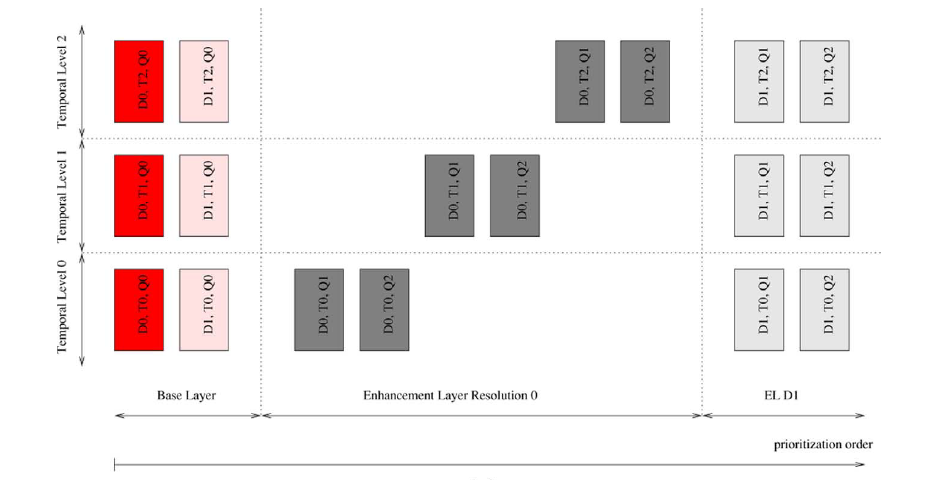
\includegraphics[width = 1.0\linewidth]{clip/06.png}
	\caption{JSVM基本截取器的算法图示\label{fig:06}}
\end{figure}

最初的参考软件JSVM提供了一个非常简单的基本截取器。该截取器并没有考虑任何优化,只是实现了一个从完整码流中丢弃一些层的包来使码率低于给定值的程序。如图\ref{fig:06}所示,该程序按照SVC中的层的概念将所有NAL数据包分成了几组,在截取丢包的时候,高层的包先丢,如果整个高层都丢弃之后仍然不能满足码率要求,再考虑丢低层的数据包。这种方法符合直观理解,因为一般来说低层的数据作为被参考对象,影响的范围更广,重要性更大一些,所以应该优先保留;反之,高层的数据可以先丢。但编码过程中形成的数据包之间的关系并没有这么简单,有可能某个高层的包比某个低层的包更重要,基本截取器并没有考虑这一点。因此,基本截取器的效果离最优还有很大的差距。此外,对于同一个层的数据包,基本截取是按某个固定的顺序依次丢弃,也并没有对这些同一层数据包的重要性做区分。这也是基本截取器效率低下的另一个原因。接下来介绍对基本截取器的改进工作。

Amonou等人\supercite{Amonou2007}提出了一个基于“Quality Layers”的码流截取方案。这一方案被SVC参考软件JSVM所采用,而且取得了比JSVM中的基本截取器更好的性能。在Amonou等人的方案中计算了一个“Quality Layers”(简称QL)值,它反映了一个数据包(NALU)的码率失真影响,据此进行截取能得到率失真优化过的结果。对于计算出来的QL值,可以用两种方法将其存储在码流中:

\begin{itemize}
\item 占用NALU头信息中的priority\_id字段来存储这个NALU的QL值。这个字段有6比特,只能存储64个不同值;
\item 用专门的补充增强信息(SEI)数据包来存储所有NALU的QL值。
\end{itemize}

在计算QL值的时候,对数据包失真影响的估计是一个计算量非常大的过程,而且估计的准确性也有提高的空间。因此,后续工作提出的失真模型一方面是降低复杂度,另一方面是进一步提高准确度。Sun等人\supercite{Sun2009}和Maani等人\supercite{Maani2009}所构造的模型都是基于帧间的误差漂移来计算失真。Sun等人的模型在性能方面几乎与JSVM相当,但计算复杂度却大大减少。而Maani等人的模型取得了比JSVM更高的估计准确度(由图\ref{fig:15}\supercite{Maani2009}可见,其估计的失真与实际失真基本相同),但是由于其是基于训练的,为了得到更鲁棒的模型参数,需要更大的计算量。

\begin{figure}[h]
	\centering
	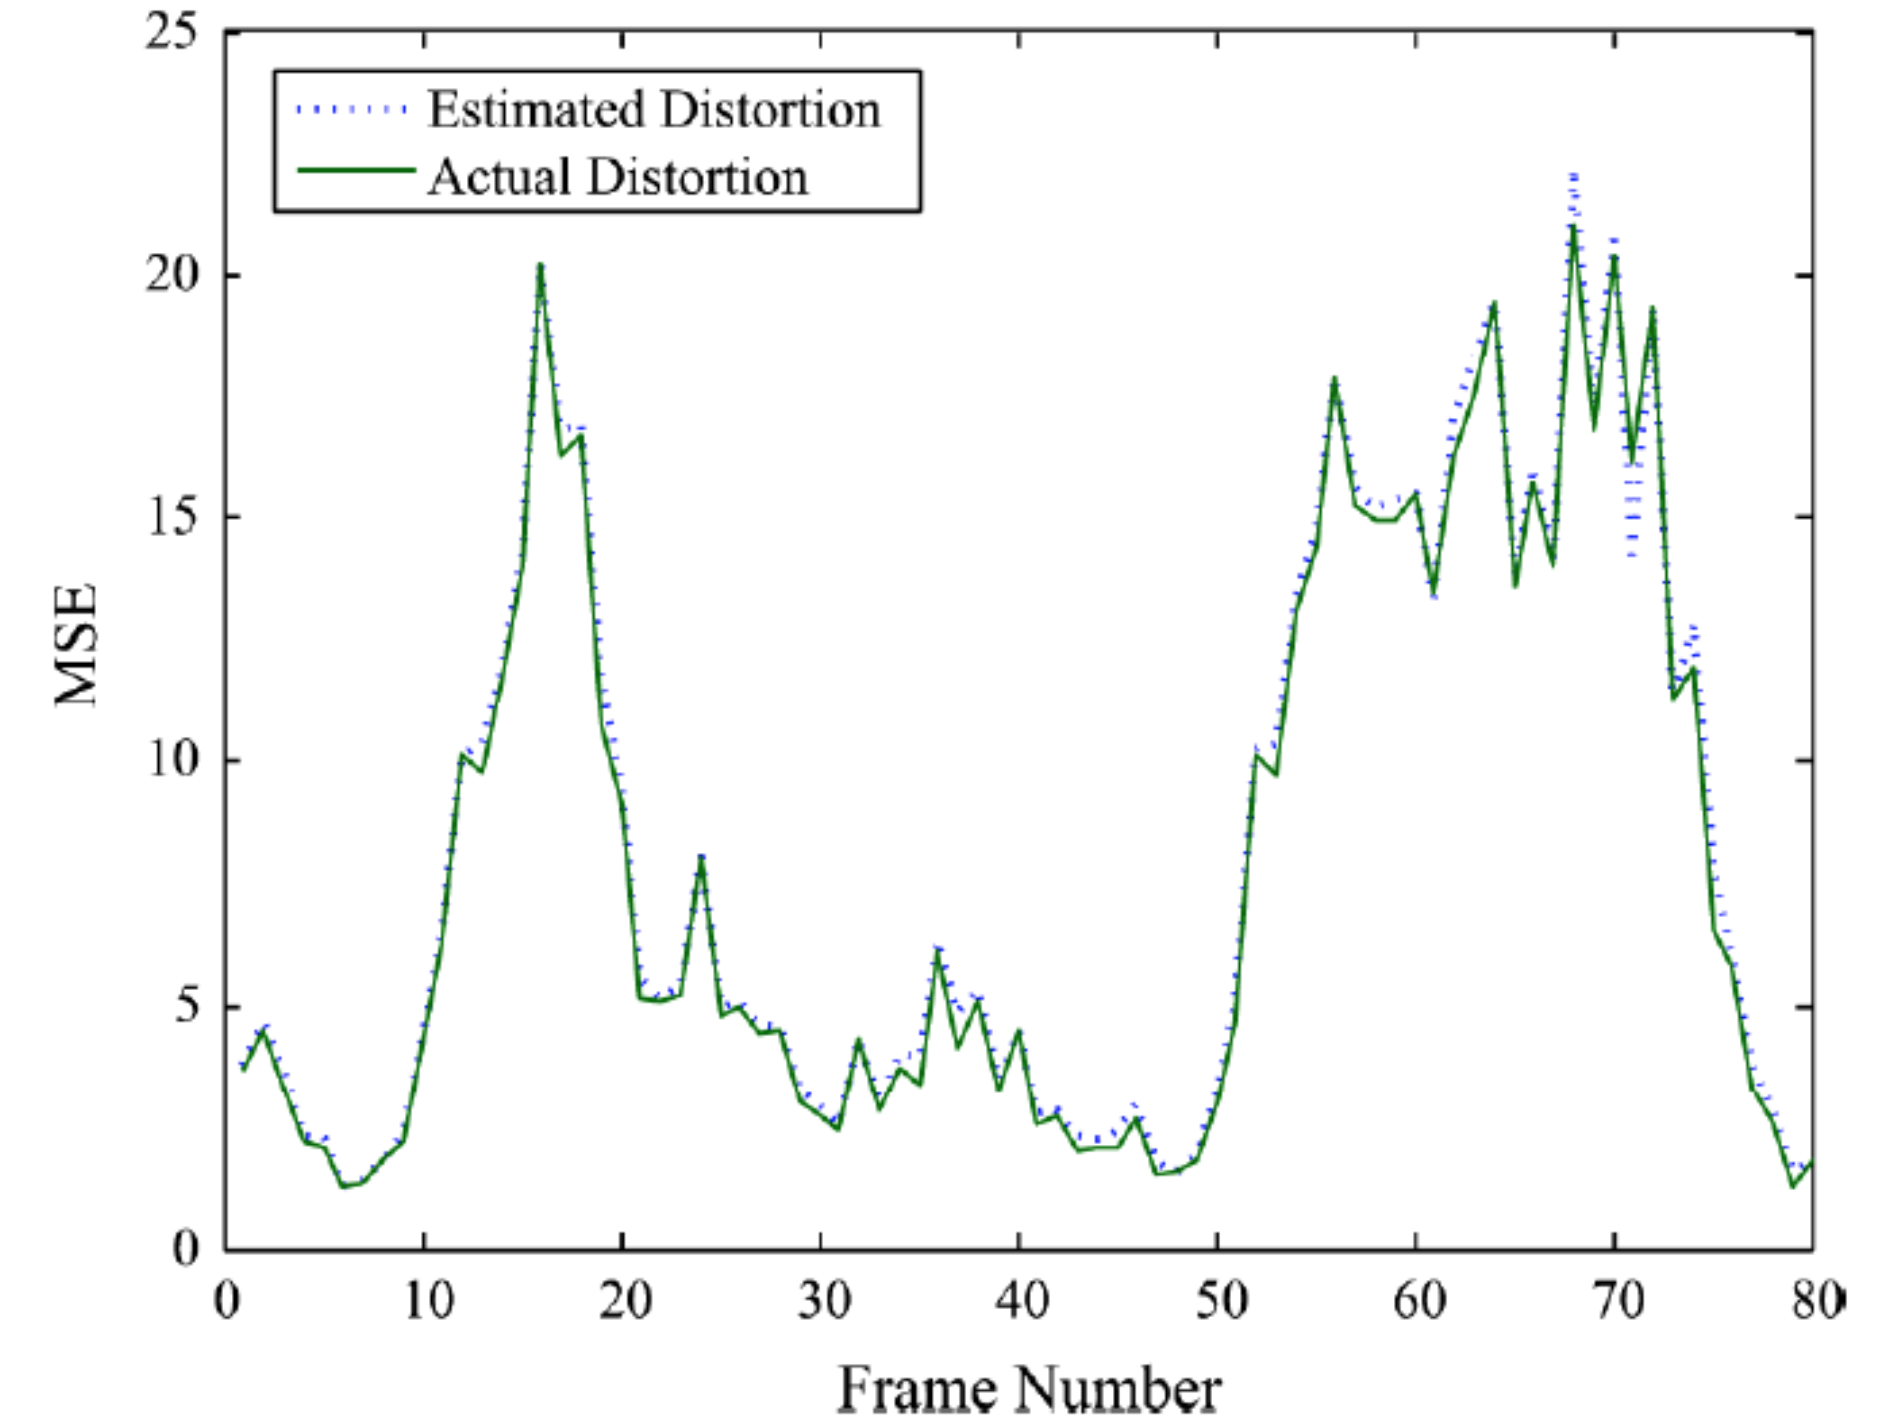
\includegraphics[width = 0.8\linewidth]{clip/16.png}
	\caption{基于训练的模型所取得的失真估计准确度图示\label{fig:16}}
\end{figure}

此外,Ramanathan等人\supercite{Ramanathan2012}提出了一个“Quality Metadata”的概念来用于码流截取,这与上面所说的“Quality Layers”是同样的思想,只是计算方法有所差别;Yang等人\supercite{Yang2013}提出了一个基于模拟退火的方法来解决码流截取问题,他们简单地用丢弃较低增强层数据带来的失真来估计丢弃较高增强层数据带来的失真。因为码流截取从另一个角度看是丢弃数据包的过程,丢弃的先后顺序可以认为是这些数据包的优先级。于是一些研究者从赋优先级的角度来提出相应的算法。例如,Lim等人\supercite{Lim2006}把可伸缩视频码流视为树形结构并据此来为每个数据包赋予优先级,而Zhu等人\supercite{Zhu2011}则采用拉格朗日乘子方法计算优先级值。在这些已有的工作中,失真估计的准确性都显著地影响最终结果。因此,提出简单有效的误差或失真模型对于码流截取的研究至关重要。本文的研究工作正是在此处着力并取得了创新性成果。


\section{传输中的码率自适应}

\subsection{问题描述}

在数据源具备码率可变的前提条件之后,实际传输时就可以根据带宽来调整发送的速率。改变码率去适应带宽的变化,这就是所谓的码率自适应问题。对于一个码率自适应算法,有三个最基本的目标。这三个目标可以用来衡量自适应算法的效果,也是设计算法时需要考虑的方面。下面分别进行描述。

对于一个流媒体系统,最首要的目标应该是保证视频播放能够连续不断。一旦视频开始播放,每个数据包都有了自己的显示时间。这个时间也决定了传输的截止时间。如果这个数据包没有在截止时间前达到客户端,那么客户端播放器就会因缺少数据而暂停。这就是用户所遇到的卡顿现象,应该努力避免。避免卡顿一般要依赖于传输中的缓冲机制。如果检测到带宽下降、当前码率确实过高,应及时下调质量,以防止数据不能按时传送而导致播放卡顿。

其次是要保持视频质量的平滑性。网络条件变化可能比较剧烈,但视频质量应该尽可能维持在一个比较稳定的水平。因为频繁的质量调整会给用户带来反感。举例来说,当用户适应了较低的质量后,突然调高质量并在短时间内又调低,给用户的体验还不如不调整。因此,在保证播放连续的前提下,应尽可能减少质量调整次数,充分利用缓冲区的作用,避免因为临时或短暂的带宽变化就调整质量。

最后,还要提供给用户尽可能好的视频质量。假设我们一直发送较低码率的视频流,那么既能保证播放的连续性又不存在平滑性的问题,上述两个目标可以轻而易举达到。但是这样的话用户看到的视频质量将一直处于较低的水平,显然不是令人满意的选择,所以不可取。码率自适应算法应该能够充分利用可用带宽,在带宽足够的情况下提高发送质量,给用户最好的观看体验。

综上所述,在视频流媒体的码率自适应研究中,保证播放流畅是最基本的要求,同时视频的高质量和平滑性也是所追求的指标。

\subsection{相关工作简介}

码率自适应的研究主要集中于如何选择和调度视频数据包。Gao等人\supercite{Gao2006}提出的调度策略首先确保重要性较高的数据优先发送,而对于重要性相同的数据包,播放时间最早的首先发送。Schier等人的工作\supercite{Schierl2010}也与此类似,把视频数据放在具有不同优先级的缓冲区中(参见图\ref{fig:15}\supercite{Schierl2010}),通过调整优先级来确保数据及时发送。在达尔文流媒体服务器中内置有一个被称为包延迟反馈的调度算法。当一个包要发送时,服务器会检测它的延时(即这个数据包应播放的时间和当前时间的差),并根据这个延时来判断当前发送顺畅还是阻塞,以此来推测带宽情况,并相应调整发送码率和质量。具体判断方法是将这个延时作为反馈,与预先设定的阈值进行比较。例如,预先决定当前带宽下发送某个数据包之后T时间内应该播放,那么理想延时应该保持为T。如果发现延时小于T了,说明发送受阻,可能是带宽减小了;反之,如果T变大了,说明发送顺畅,可以考虑增加质量。这种算法能够在一定程度上检测带宽的变化并作相应调整。但是它的调整策略是保守的,在它检测到延时变小时,很可能客户端已经因为缺少数据而停止了。而且该算法对带宽的变化趋势也不能提前预测,很可能导致质量波动,这也是需要改善的一个问题。

\begin{figure}[t]
	\centering
	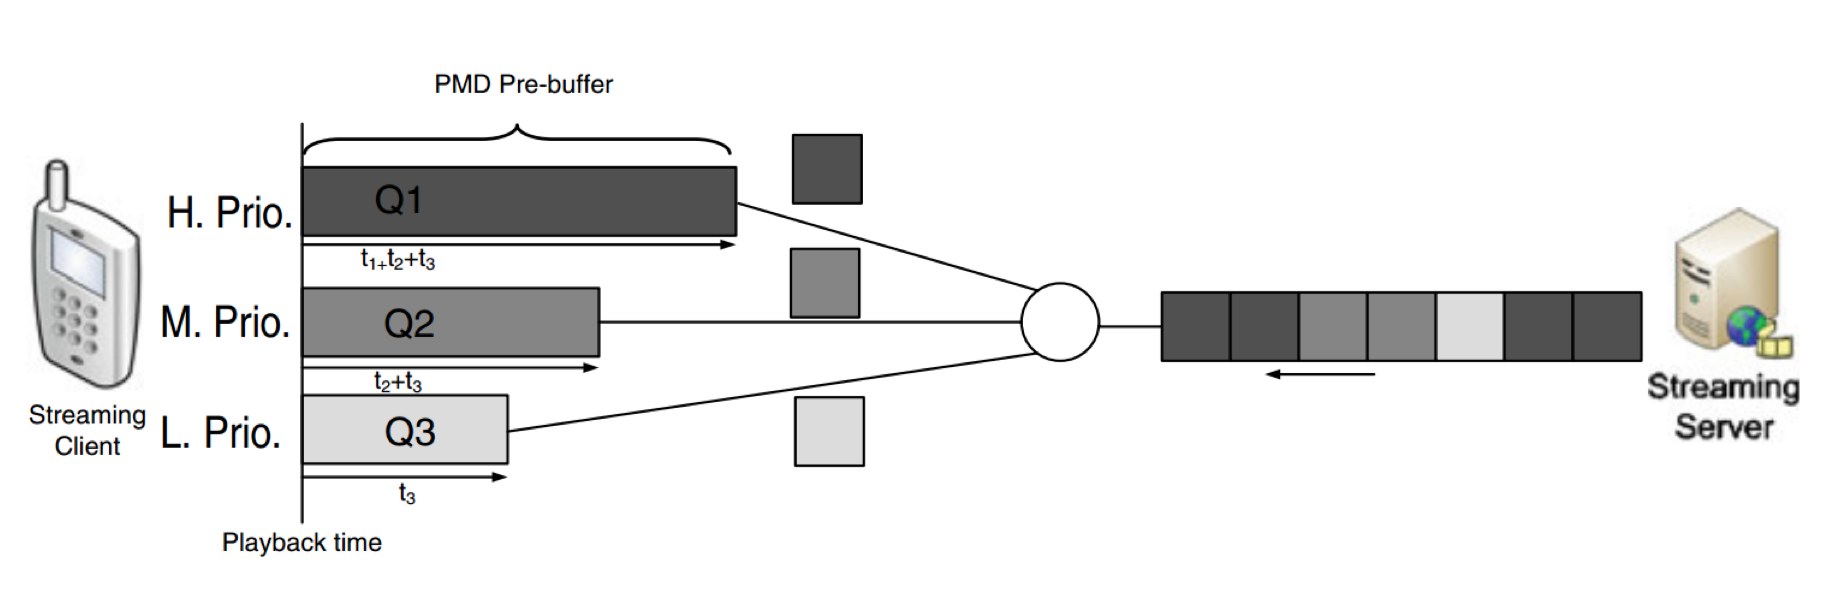
\includegraphics[width = 1.0\linewidth]{clip/15.png}
	\caption{基于不同优先级缓冲区的码率自适应算法\label{fig:15}}
\end{figure}

上面的工作都是针对可伸缩视频流媒体系统或是RTSP传输协议进行的。对于HTTP动态自适应流媒体(DASH),国内外也已经有了不少研究。例如,Akhshabi等人\supercite{Akhshabi2012}分析了来自商业公司和开源社区的多个DASH客户端播放器的自适应行为,比较了他们之间性能的优缺点。张辉帅等人\supercite{Zhang2013}提出了一种基于拉模式的码率自适应算法,利用滑动窗口分析最近若干分片的下载时间,基于此来选择最合适的码流。Huang等人\supercite{Huang2015}结合了缓冲区的状态和对带宽容量的估计这两个判据来做如何调整码率的决策。Juluri\supercite{Juluri2015}等人考虑到每个分片数据量大小不同可能导致下载时间的差异,因此提出了一种提前查看分片信息的码率自适应算法。

这些已有的研究工作在一定程度上提高了传输效果,但大都是针对点播模式,没有考虑到直播模式下的特殊问题。目前实时性直播的应用越来越广,从某种程度上来说是一个更重要的模式。直播由于其数据是实时产生的,无法提前加载,因此与点播有所不同,需要进行针对性的研究,设计新的码率自适应算法。本文的工作不仅适用于点播系统,也能很容易扩展应用到直播系统中。

\section{视频解码优化}

视频解码器优化的工作总是紧密结合视频编码标准而进行。本文主要关注最新的国际视频编码标准HEVC的相关工作。自HEVC推出以来,不少论文都针对其解码器实现和优化进行了研究。大部分已公开的研究工作都是在标准化组织所提供的参考软件HM\supercite{HM}的基础上进行的。在HM之外,我们所能查到的在正式发表文献中提出的独立解码器实现只有少数几个\supercite{Bossen-TCSVT2012,JCTVC-G988,JCTVC-H0693}。除了外在的性能报告和复杂度分析,这些文献中既没有给出任何技术细节或者源代码,也没有提供可以公开测试的演示程序。因此它们对HEVC的实际应用贡献并不大。Chavarrias等人\supercite{Chavarrias-TCE2013}提出了一个新的基于数字信号处理器(DSP)的HEVC解码器。但由于不是针对通用处理器平台,其应用局限性也比较大。本文研究的是在x86和ARM架构的通用处理器上的解码优化。下面分数据级和任务级两个方面对相关的工作进行介绍。

\subsection{数据级优化工作}

数据级解码器优化主要是采用单指令多数据(Single Instruction Multiple Data,SIMD)的处理器指令集扩展来对解码过程中的特定计算模块进行加速。SIMD所适用的主要是运动校正、整数变换、去块滤波这些计算密集而规整的模块。不同编解码标准对这些模块的定义并不完全相同。就HEVC而言,它在运动校正时采用了8抽头的基于DCT的插值\supercite{JCTVC-F537},而且在去块滤波之后加入了一个称为采样自适应偏移(Sample Adaptive Offset,SAO)的新操作\supercite{Fu-TCSVT2012}。由于SIMD算法的设计与这些模块的操作密切相关,因此针对以前标准设计的数据级解码优化算法\supercite{Casalino-ICMCS1999,Lappalainen-TCSVT2003,Malvar-TCSVT2003,Chen-JVCIR2006,Pescador-TCE2009}都不再适用于HEVC。Yan等人\supercite{Yan-VCIP2012}在HM 4.0的基础上,采用SIMD技术对一些解码模块进行了加速。但随着标准文档和参考文件的更新,最终版本的HEVC相对于HM 4.0有些模块发生了变化,例如上述工作中所加速的自适应滤波\supercite{JCTVC-F303}最终被从标准中移除。因此,针对最新的标准需要重新设计和实现数据级的优化算法。

\subsection{任务级优化工作}

任务级解码器优化主要是通过多线程来并行执行解码任务,以充分利用多核CPU的并行特性。HEVC标准在设计的时候考虑了对任务级并行的支持,引入了分片(tiles)\supercite{JCTVC-E408}和波阵面并行处理(Wavefront Parallel Processing,WPP)\supercite{JCTVC-E196}这两种技术。它们能够将解码分成互相独立的任务来同时执行,一定程度上可以提高整体解码速度。Chi等人\supercite{Chi-TCSVT2012}还基于WPP提出了一个称为“overlapped wavefront”的任务级并行优化技术,对于用WPP编码的视频码流取得了期望的解码加速比。然而需要指出的是,分片和WPP都是HEVC标准中的可选配置,如果视频码流在编码的时候没有开启这些选项,那么解码器就无法利用这两个新特性。从实用的角度来看,采用不依赖于这些特殊配置的帧级并行解码结构才具有更广泛的意义。这也正是本文工作所选择的方向。

\section{本章小结}

本章首先对视频的压缩编码和流式传输做了介绍,其中包含了本文研究工作的知识基础;然后结合本文的研究内容对码流截取、码率自适应、解码器优化这几个方面的问题和已有工作进行了概述。后续章节将对这几个问题依次进行研究,提出相应的方案和算法,并展示实验结果。